\documentclass{article}
\usepackage{graphicx}
\usepackage{wrapfig}
\usepackage{subcaption}
\usepackage[margin=1in]{geometry}
\usepackage{amsmath} % or simply amstext
\usepackage{amssymb}
\usepackage{siunitx}
\usepackage{booktabs}
\usepackage[export]{adjustbox}
\newcommand{\angstrom}{\textup{\AA}}
\newcommand{\colormap}{jet}  % colorbar to use
\usepackage{cleveref}
\usepackage{booktabs}
\usepackage{gensymb}
\usepackage{float}

\title{Using Stochastic Modeling to Predict Long Timescale Transport Behavior of Solutes in an H\textsubscript{II} Phase Lyotropic Liquid Crystal Membrane}
\author{Benjamin J. Coscia \and Michael R. Shirts} 

\begin{document}

  \graphicspath{{./figures/}}
  \maketitle

  \section{Introduction}

  We need highly selective membranes in order to perform efficient separations.

  Amphiphilic molecules are capable of self-assembling into ordered nanostructures.

  Lytropic liquid crystals are a class of amphiphilic molecules that can be cross-linked
  into mechanically strong membranes.
  \begin{itemize}
  	\item H\textsubscript{II} phase lyotropic liquid crystals have densely packed, uniform
	sized pores and have the potential to disrupt conventional membrane separation
	techniques by being selective based not only on size and charge, but on chemical
	functionality as well.
	\item Q\textsubscript{I} phase LLCs consist of a tortuous network of 3D interconnected
	pores.
  \end{itemize}

  We can only learn so much from experiment. MD can give us mechanistic insights with
  atomistic resolution so that we can intelligently design new membranes for 
  solute-specific separations.

  In our previous work, we studied the transport of 20 small polar molecules
  in an H\textsubscript{II} phase LLC membrane. 

  Unfortunately, the timescales that we can simulate with MD are insufficient to be
  able to predict well-converged predictions of macroscopic transport properties 
  traditionally used to characterize membranes in the lab.

  % review of techniques for predicting long time scale behavior

  In this work, we explore two approaches to modeling the dynamic behavior of 
  a subset of solutes that we studied in our previous work.
  \begin{itemize}
  	\item First is based on the anomalous diffusion literature
  	\item Our second approach to modeling solute transport groups solute behavior
    into different dynamical states.
%  	\item Second focuses on the analysis of time series  % Need a better way to talk about it here 
  \end{itemize}

  \section{Methods}
    
  We ran all MD simulations and energy minimizations using GROMACS 2018. We
  performed all post-simulation trajectory using python scripts which are available
  online at \texttt{https://github.com/shirtsgroup/LLC\_Membranes}.

  \subsection{Molecular Dynamics Simulations}

  We studied transport of solutes in the H\textsubscript{II} phase using an
  atomistic molecular model of four pores in a monoclinic unit cell with 
  10 \% water by weight. 
  \begin{itemize}
    \item Approximately one third of the water molecules occupy the tail region 
    with the rest near the pore center.
    \item We chose to study the 10 wt \% water system because solutes move 
    significantly faster than in the 5 wt \% system studied previously.
    \item Appropriate stochastic modeling requires that solutes explore 
    as much structural space as possible.  %BJC: better term than structural space?
  \end{itemize}
  
  We chose to study a subset of 4 of the fastest moving solutes from our previous
  work: methanol, acetic acid, urea and ethylene glycol.
  \begin{itemize} 
    \item In addition to exploring membrane structural space the most, these solutes
    have a relatively diverse set of chemical functionality.   
    \item For each solute we created a separate system and to each system we
    added 6 solutes per pore for a total of 24 solutes.
    \item This number of solutes per pore provides a balance of a low 
    degree of interaction between solutes and sufficient amount of data from
    which to generate statistics on the time scales which we simulate.
    \item Further details on the setup and equilibration of these systems can
    be found in our previous work.\cite{coscia_chemically_2019}
  \end{itemize}
  
  We extended the 1 $\mu$s simulations of our previous work to 5 $\mu$s in order
  to collect ample data.
  \begin{itemize}
    \item We simulated the system with a time step of 2 fs at a pressure of 1 bar
    and 300 K controlled by the Parinello-Rahman barostat and the v-rescale thermostat
    respectively.
  \end{itemize}
  
  \subsection{Modeling subdiffusion}\label{method:model_sFBM}

  Solutes in our H\textsubscript{II} LLC membrane system exhibit subdiffusive
  behavior, a type of anomalous diffusion.
  \begin{itemize}
  	\item During an anomalous diffusion process, the mean squared displacement (MSD)
  	does not grow linearly with time, rather it is of the form:
	\begin{equation} 
	\langle x^2(t) \rangle = K_{\alpha}t^\alpha
	\label{eqn:msd_form}
	\end{equation} 
	where $\alpha$ is the anomalous exponent and $K_\alpha$ is the
	generalized diffusion coefficient.
	\item A value of $\alpha < 1$ indicates a subdiffusive process, while values of
	$\alpha = 1$ and $\alpha > 0$ are characteristic of Brownian and superdiffusive
	motion respectively.
  \end{itemize}

  \noindent We analyzed both the ensemble-averaged and time-averaged MSDs
  of the simulated trajectories.
  \begin{itemize}
	\item The ensemble-averaged MSD measures the displacement of a particle from its initial
	position~\cite{meroz_toolbox_2015} and can be written as
	\begin{equation}
	\langle x^2(t) \rangle = \langle x(t) - x(0) \rangle
	\label{eqn:ensemble_msd}
	\end{equation}
%	\item The average MSD calculated in this way recovers the form of
%	Equation~\ref{eqn:msd_form}. % time-averaged should recover it too for FBM 
	\item The time-averaged MSD measures the displacement between all possible time lags
	and can be written as
	\begin{equation}
	\overline{x^2(\tau)} = \dfrac{1}{T - \tau}\int_{0}^{T - \tau} (x(t + \tau) - x(t))^2 dt
	\end{equation}
	where $\tau$ is the time lag and T is the length of the
	trajectory~\cite{meroz_toolbox_2015}. 
  \end{itemize}
  
  \noindent Three common mathematical models for modeling anomalous subdiffusion
  processes include continuous time random walks (CTRW), fractional Brownian motion
  (FBM) and random walks on fractals (RWF).\cite{meroz_toolbox_2015}
  \begin{itemize}
    \item FBM is common in crowded, viscoelastic environments where each step comes 
    from a Gaussian distribution but is anti-correlated to its previous 
    step.~\cite{mandelbrot_fractional_1968,jeon_fractional_2010,banks_anomalous_2005}
    \item A CTRW is characterized by a distribution of hop lengths and 
    dwell times, where each each step is characterized by independent random draws from 
    each distribution.\cite{montroll_random_1965,morrin_three_2018}
    \item An RWF is imposed by a system's geometry. Systems with tortuous pathways and dead
    ends cause anti-correlated motion.\cite{meroz_toolbox_2015,neusius_subdiffusion_2008}
    \item The processes described above can happen alone or in combination.  	
  \end{itemize}
  
  % BJC: Should this be in the results?
  \noindent We believe that solutes in the system studied here exhibit subordinated 
  fractional Brownian motion (sFBM) where the parent process is FBM and the 
  leading process is a CTRW. 
  \begin{itemize}
  	\item The ensemble-averaged MSD differs from the time-averaged MSD, which
  	is indicative of non-ergodicity, a trait inherent to CTRWs but not FBM or RWFs.~\cite{thiel_weak_2014}
  	\item We also observe non-stationary $z$-coordinate traces of each solute's
  	center of mass (COM). %BJC: figure of a z-coordinate trace in main text or in supporting info
  	\item For a pure CTRW, the time-averaged MSD should be linear.
  	~\cite{neusius_subdiffusion_2008,meroz_subdiffusion_2010}
  	\item However, a typical time-averaged solute MSD is sublinear (see supporting
  	information), which suggests that there is another underlying subdiffusive mechanism.
  	\item The hop lengths recorded after each dwell period are anti-correlated (See supporting information)
  	\item Given the viscoelastic nature of the monomers in our system, we believe
  	the hop lengths can be modeled with FBM. 
 	\item For subordinated FBM, it can be shown that
  	\begin{equation}
  	\langle x^2(t) \rangle \simeq t^{\alpha\beta}
  	\end{equation}
  	where $\alpha$ is the anomalous exponent characteristic of the leading CTRW process
  	and $\beta$ is the anomalous exponent characteristic of the parent FBM process. 
  \end{itemize}

  \noindent We can characterize a CTRW process using the parameters which describe its
  dwell time and hop length distribution.
  \begin{itemize}
	\item We used the \texttt{ruptures} python package in order to identify
	changepoints in solute trajectories.\cite{truong_ruptures:_2018} (See Supporting
	Information for more details on chosen parameters. i.e. type of cost function, 
	cost function penalty tolerance, number of dimensions used)
	\item We used the corresponding hop lengths and dwell times between break points
	to construct empirical distributions.
  \end{itemize}
	
  For solutes in our system, the distribution of hop lengths appears to be
  well-represented by a Gaussian distribution.~\cite{metzler_random_2000,
  metzler_anomalous_2014,neusius_subdiffusion_2009}
  \begin{itemize}
	\item We are most interested in the standard deviation, $\sigma$, of the 
	hop length distribution.
  \end{itemize}
  
  The distribution of dwell	times is expected to fit a power law (or heavy-tailed)
  distribution proportional to $t^{-1-\alpha}$.~\cite{meroz_toolbox_2015}
  \begin{itemize}
	\item Because we are limited to taking measurements at discrete values
	dictated by the output frequency of our simulation trajectories, we fit the
	empirical dwell times to a discrete power law distribution whose maximum
	likelihood $\alpha$ parameter we calculated by maximizing the following
	likelihood function: 
        \begin{equation}
	\mathcal{L}(\beta) = -n\text{ln}\zeta(\beta, x_{min}) -
	\beta\sum_{i=1}^{n} \text{ln}~x_i 
	\label{eqn:powerlaw_likelihood}
	\end{equation}
	where $\beta = 1 + \alpha$, $x_i$ are collected dwell time data points,
	$n$ the total number of data points, and $\zeta$ is the Hurwitz zeta function
	where $x_{min}$ is the smallest measured value of
	$x_i$.~\cite{clauset_power-law_2009} 
	\item We obtained distributions of the hop length standard deviations, $\sigma$, and
	$\alpha$ using statistical bootstrapping.\cite{efron_introduction_1994} 
  \end{itemize}
  
  \noindent FBM processes can be described using the Hurst parameter, $H$, where 
  $H = \beta/2$.
  \begin{itemize}
  	\item Brownian motion is recovered for $H = 0.5$
	\item The autocovariance function of hop lengths has the analytical form:~\cite{mandelbrot_fractional_1968}
    \begin{equation}
	\gamma(k) = \dfrac{1}{2}\bigg[|k-1|^{2H} - 2|k|^{2H} + |k+1|^{2H}\bigg]
	\label{eqn:autocovariance}
	\end{equation}
	where $k$ is the number of increments between hops.
	\item We obtained H by performing a least squares fit of Equation~\ref{eqn:autocovariance}
	to the empirically measured autocovariance function.
	\item We used statistical bootstrapping to generate a distribution of $H$ 
	values. %BJC: can provide more detail in supporting or just reference python script
  \end{itemize}
  
  In general, we observe different dynamical behavior when solutes move inside the
  pore versus in the tail region.
  \begin{itemize}
    \item Therefore, we created 2 sets of parameters based on the solute's radial location.
    \item Solutes in the pore region are located less than 0.75 nm from the pore center and
    all else are in the tail region. 
    \item We determined this cut-off and described how we calculated radial 
    distance from the pore center in our previous work~\cite{coscia_chemically_2019}
  \end{itemize}

%  We generated distributions of parameters for the dwell time and hop length
%  distributions using statistical bootstrapping.
%  \begin{itemize}
%	\item For each type of distribution, we randomly selected $n$ data points from the empirical
%	distribution with replacement.
%	\item We repeated the fitting procedure described above for each of 200 bootstrap trials.
%  \end{itemize} 

%  We calculated macroscopic diffusion coefficients by simulating trajectories orders of
%  magnitude longer than our molecular simulations.
  \noindent For each solute, we simulated 10000 5 $\mu$s sFBM trajectories. 
  \begin{itemize}
	\item We constructed trajectories by simulating	sequences of dwell times and correlated 
	hop	lengths generated based on parameters randomly chosen from our bootstrapped parameter
	distributions.
	\item We propagated each trajectory until the total time reached 1 $\mu$s, and truncated
	the last data point so that the total time exactly equaled 5 $\mu$s. 
    \item Valid comparisons are only possible between fixed length sFBM simulations. The
    power law dwell time behavior gives rise to the aging phenomenon, embodied by
    a decrease in MSD with measurement time.~\cite{neusius_subdiffusion_2008,metzler_anomalous_2014}
    \item We reported the MSD after 5 $\mu$s with corresponding 95 \% intervals
% Following probably better suited for supporting information, if included at all
%	\item We randomly sample Gaussian hop lengths using the
%	\texttt{numpy.random.normal} method of the \texttt{numpy} python package.
%	\item We randomly sampled dwell times from a discrete power law
%	distribution based on the recommendations of Clauset et
%	al.~\cite{clauset_power-law_2009}: 
%	\begin{equation}
%	x = \lfloor
%	(x_{min} - \tfrac{1}{2})(1 - r)^{-1/(\alpha - 1)} + \tfrac{1}{2} \rfloor
%	\label{eqn:discrete_powerlaw_draws}
%	\end{equation}
%	where $r$ is randomly drawn from a uniform distribution which we simulated
%	with \texttt{numpy.random.uniform}.
%	\item We found that thermal noise does not significantly influence the MSD and
%	therefore did not add any noise to the simulated trajectories. (See supporting info)
  \end{itemize}

%BJC: probably don't need to explain this in great detail
%  \noindent We fixed the length of each simulated trajectory so that we could compare the total
%  MSD between different solutes without the influence of the ageing phenomenon.
%  \begin{itemize}
%	\item Ageing is defined by the tendency of the average MSD to decrease
%	as the length of trajectories are increased~\cite{metzler_anomalous_2014}.
%	\item The maximum measured dwell time can be no longer than the total length
%	of a simulated trajectory. 
%	\item As measurement time or trajectory length is increased, longer dwell times
%	are incorporated into the calculation, lowering the average MSD. (See supporting
%	info for demonstration)
%	\item We can achieve consistent total MSDs with low uncertainty for
%	simulated trajectories created with a given set of parameters if we fix the
%	trajectory length (as opposed to total number of steps).  
%  \end{itemize}

%  \subsubsection*{Coordination number}

%  We quantified the coordination of solutes with surrounding molecules.
%  \begin{itemize}
%  	\item For each frame, we counted the identities and number of
%  	coordinated molecules to a given solute based on a distance cut-off. 
%	\item We found that this approach is more useful than calculating the
%	3D spherical radial distribution function because it gives detailed
%	frame-by-frame information rather than an average. 
%  \end{itemize}

  \subsection{The Infinite State Hidden Markov Model}  %BJC: potentially a separate paper
  
  Hidden Markov models (HMMs) are a useful and widely used technique
  for modeling sequences of observations where the probability of the next observation
  in a sequence depends only on a previous unobserved, or hidden, state.~\cite{beal_infinite_2002}
  \begin{itemize}
    \item In the context of our simulations, the observations correspond to 
    the center of mass coordinates of the solutes versus time, and the states
    correspond to the dynamical behavior which give rise to those types
    of observations.
    \item Unfortunately, standard HMMs require the number of hidden states to be known
    a priori.
  \end{itemize}
  
  The infinite-state HMM overcomes this drawback by placing a hierarchical
  Dirichlet process (HDP) prior on the transition probabilities.
  \begin{itemize}
    \item Using some base probability distribution, H, a Dirichlet process 
    (DP) generates distributions over a countably infinite number of 
    probability measures:
    \begin{equation}
      G_0 = \sum_{k=1}^{\infty} \beta_k \delta_{\theta_k} ~~ \theta_k \sim H, \beta \sim GEM(\gamma)
    \end{equation}
    where the $\theta_k$ are values drawn from the base distribution and the
    weights $\beta_k$ come from a stick-breaking process parameterized by the concentration 
    parameter $\gamma$ (equivalently referred to as GEM($\gamma$)). 
    \item The concentration parameter expresses one's confidence in H relative to the posterior 
    and is closely related to the number of data observations.
    \item Each row, $G_j$, of the transition matrix is produced by drawing from a DP specified 
    using the $\beta$ vector as a discrete base distribution and a separate concentration
    parameter, $\alpha$.
    \begin{equation}
      G_j = \sum_{k=1}^{\infty} \pi_{jk} \delta_{\theta_k} ~~ \pi_j \sim DP(\alpha, \beta)
    \end{equation}
    \item This hierarchical specification ensures that the transition probabilities in 
    each row share the same support points \{$\theta_1$, ..., $\theta_k$\}.
  \end{itemize}
   
  \noindent We describe the dynamics of each state using a vector autoregressive (VAR) model. 
  \begin{itemize}
  	\item A VAR process is characterized by a vector of observations in a time series 
  	that are dependent on $r$ previous values of the time series vector, weighted by a
  	coefficient matrix $A_i$ in addition to a white noise term $\mathbf{e}_t$:
  	\begin{equation}
  	\mathbf{y}_t = \sum_{i=1}^r A_i\mathbf{y}_{t-i} + \mathbf{e}_t~~~~\mathbf{e}_t \sim N(0, \Sigma)
  	\end{equation}
  	\item We assumed multivariate Gaussian noise and limited our analysis to an 
  	autoregressive order of $r=1$.
  	\item We used a conjugate matrix-normal inverse-Wishart prior on parameters
  	$A$ and $\Sigma$ in order to analytically draw from the posterior.
  \end{itemize}   
  
  Based on the VAR parameters and matrix of transition probabilities, we calculated
  the most likely sequence of hidden states.
  \begin{itemize}
    \item We repeated this process iteratively until we reached convergence % BJC: need to define convergence criteria
    \item Our python implementation of this process is heavily adapted from the MATLAB code
    of Fox et al.~\cite{fox_sticky_2007} 
    \item We refer the interested reader to much more extensive descriptions of 
    this process and its implementation. 
    ~\cite{beal_infinite_2002,teh_hierarchical_2006,van_gael_beam_2008,fox_nonparametric_2009,fox_bayesian_2010}
  \end{itemize}
   
  \section{Results and Discussion}

  \subsection{Subordinated Fractional Brownian Motion Modeling}\label{section:sFBM}
  
  %BJC: focus on MD MSD results
  \noindent We calculated the MSD of each solute in the set over the course of 1$\mu$s MD simulations.  %BJC: type of MSD TBD 
  \begin{itemize}
	\item We extracted values of $\sigma$, $\alpha$ and $H$ for each solute
	and then simulated 10000 sFBM trajectories of the same length as our MD
	simulations, as described in Section~\ref{section:model_sFBM} of the Methods.
	\item The final MSDs of the sFBM trajectories are compared to those 
	calculated directly from MD simulations in Figure~\ref{fig:all_msds}. 
	\item The three sFBM parameters, calculated based on MD solute trajectories
	are presented in Table~\ref{table:simulations}.
	\item We would like to emphasize that we rely on the MD MSD values in order to
	define trends in the total MSD, while the sFBM trajectories and parameter 
	values allow us to speculate as to the reasons for the observed trends. 
	\item There is a non-negligible amount of error in the calculation of 
	each parameter which prevents us from reliably portraying our sFBM MSDs as
	reduced	uncertainty MD MSDs.
  \end{itemize}
  
  % BJC: worth including single parameter model (i.e. no radial dependence) to 
  % show its shortcomings? Or send to supporting information
  \begin{table}[h]
  \centering
  \begin{tabular}{cccc}
  \toprule
  System & $\sigma$ ($nm$) & $\alpha$ & $H$ \\
  \midrule
  Methanol & 0.46 & 0.85 & 0.40 \\
  Urea & 0.33 & 0.64 & 0.40 \\
  Ethylene Glycol & 0.35 & 0.64 & 0.36 \\
  Acetic Acid & 0.28 & 0.51 & 0.44 \\
  \bottomrule
  \end{tabular}
  \caption{We calculated values $\sigma$, $\alpha$ and $H$ from MD simulation
  trajectories and then computed the average ensemble-averaged MSD of 10000 
  simulated trajectories.}\label{table:simulations}
  \end{table}
  
  Our simulated sFBM MSDs qualitatively reproduce the MD trends.
  \begin{itemize}
    \item sFBM generally lower
    \item There are a few noticeable discrepancies.
    \item We will discuss reasons for these as we proceed with the discussion.
  \end{itemize}

  \begin{figure}
  \centering
  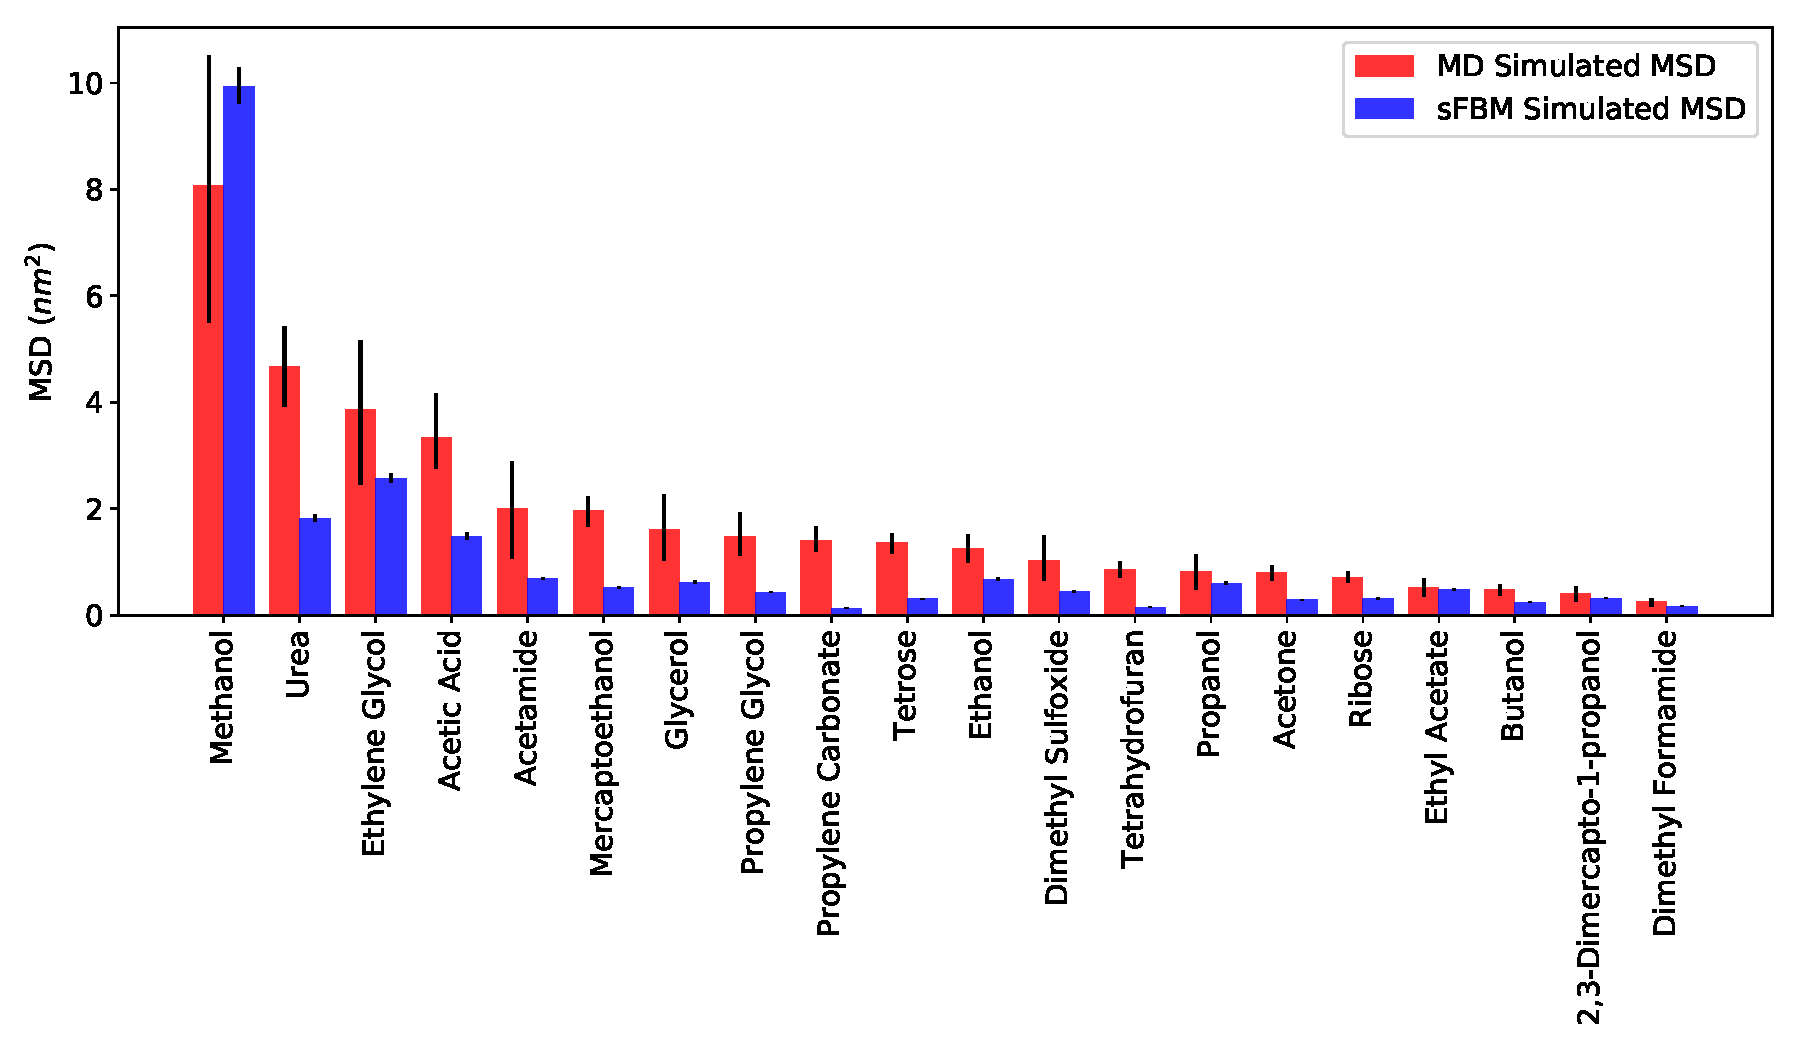
\includegraphics[width=\textwidth]{all_emsds.pdf}
  \caption{}\label{fig:all_msds}
  \end{figure}

  It most cases, it is easy to relate $\sigma$, $\alpha$ and $H$ to the
  simulated MSD values presented in Table~\ref{table:simulations}. 
  \begin{itemize}
  	\item Higher values of $\sigma$ indicate larger average hop lengths.
  	\item Higher values of $\alpha$ mean that there will be less sampling of 
  	long dwell times.
  	\item Values of $H$ near the Brownian limit of 0.5, indicate a lower degree
  	of anti-correlation.
  	\item All of which contribute to an overall increase in the simulated MSD
  \end{itemize}

  % BJC: figure with selected trajectories for each molecule.
  We fit a CTRW model (see Section~\ref{method:CTRW}) to these 
  trajectories and predicted macroscopic diffusion coefficients which are
  presented in Table TBD.
  \begin{itemize}
	\item We confirmed that our molecules exhibit anomalous diffusion
	by fitting a power law to the MSD curve. The exponent is less than
	1, indicative of anomalous subdiffusion.
	\item We used the decision making process given by Meroz and Sokolov
	in order to identify the appropriate subdiffusion model to use 
	based on our time series (See Section S-TBD of the Supporting info for
	more details).
	\item The motion of the solutes is non-ergodic and the steps are
	uncorrelated which tells us the system is likely well-described
	by a CTRW. 
  \end{itemize}
  
  \section{Markov Modeling}\label{section:markov_models}

  \section{Conclusion}
 
  \section*{Supporting Information}

  Detailed explanations and expansions upon the results and procedures mentioned in
  the main text are described in the Supporting Information. This information is
  available free of charge via the Internet at http://pubs.acs.org.

  \section*{Acknowledgements}

  Molecular simulations were performed using the Extreme Science and
  Engineering Discovery Environment (XSEDE), which is supported by National
  Science Foundation grant number ACI-1548562. Specifically, it used the Bridges
  system, which is supported by NSF award number ACI-1445606, at the Pittsburgh
  Supercomputing Center (PSC). This work also utilized the RMACC Summit supercomputer,
  which is supported by the National Science Foundation (awards ACI-1532235 and
  ACI-1532236), the University of Colorado Boulder, and Colorado State
  University. The Summit supercomputer is a joint effort of the University of
  Colorado Boulder and Colorado State University.

  \clearpage

  \bibliographystyle{ieeetr}
  \bibliography{stochastic_transport}

  \newpage

  \section*{TOC Graphic}

\end{document}
